\documentclass[pdftex]{beamer}
%\documentclass[notes=show]{beamer}
%\documentclass[xcolor=dvipsnames]{beamer}

\usepackage{amssymb}
\usepackage{latexsym}
\usepackage{amsfonts}
\usepackage{amsmath}
\usepackage[absolute,overlay]{textpos}
\usepackage[english]{babel}
\usepackage[latin1]{inputenc}
%\usepackage{times}
\usepackage[T1]{fontenc}
\usepackage{tabularx}
\newcolumntype{Y}{>{\small\raggedright\arraybackslash}X}
\usepackage{graphicx}
\usepackage{bigstrut}
\usepackage{bbm}
\usepackage{mathrsfs}
\usepackage{epsfig}
\usepackage{array}
%\usepackage{natbib}

\mode<presentation> {
%\usetheme[left,width=1.7cm]{Berkeley}
%\usetheme{default}
\usetheme{Boadilla}
  \usecolortheme[RGB={103,102,204}]{structure}
%\usecolortheme{dove}
  \useoutertheme{infolines}
  \setbeamercovered{transparent}
 }

%\renewcommand{\familydefault}{cmss}
%\renewcommand{\mathrm}{\mathsf}
%\renewcommand{\textrm}{\textsf}
\usefonttheme{serif}
\newcommand{\plim}{\mathrm{\,plim\,}}
\newcommand{\mean}{\mathrm{\,mean\,}}
\newcommand{\htn}{\hat{\theta}_{n}}
\newcommand{\mysp}{\hspace{2em}}

\newcommand{\X}{{\mathbf{X}}}
\newcommand{\x}{{\mathbf{x}}}
\newcommand{\E}{\mathsf{E}}
\newcommand{\V}{\mathsf{Var}}
\setbeamercolor{bibliography entry title}{fg=black} \setbeamercolor{bibliography entry author}{fg=black} \setbeamercolor{subsection in
toc}{fg=structure} \setbeamercolor{palette primary}{bg=structure, fg=white}
%\setbeamercolor{palette secondary}{bg=structure, fg=black}
%\setbeamercolor{palette tertiary}{bg=structure, fg=black}
\setbeamercolor{caption name}{fg=black} \setbeamersize{text margin left=.8cm} \setbeamersize{text margin right=1cm}
\hypersetup{linkbordercolor={1 0 0}} \setbeamertemplate{navigation symbols}{} \setbeamertemplate{headline}[default]

\setbeamertemplate{enumerate items}[default]

\newcounter{transfct}
\newcounter{begbs}
\newcounter{endbs}
\title[Limited Dependent Variables]{Econometrics 2}

\author[Lychagin \& Mu\c co]{Sergey Lychagin}
\institute[CEU]{Central European University}
\date{Winter 2020}

\AtBeginSection[] {
  \begin{frame}<handout:0>
    \frametitle{TOC}
    \tableofcontents[currentsection]
  \end{frame}
}


\pgfdeclareimage[height=.7cm]{logo}{rgs2} \logo{\pgfuseimage{logo}}

\begin{document}

\frame{\titlepage}





\begin{frame}
\frametitle{Types of Dependent Variables}

\begin{description}
  \item[Continuous] A continuous variable is one which can take on infinitely many, uncountable values.
    \item[Discrete] The number of permitted values is either finite or countably infinite.
\begin{itemize}\scriptsize
  \item Binary: $Y \in \{0,1\}$ \emph{qualitative} interpretation, e.g. go to college, take a job, buy a product ...
  \item Multinomial: outcome of a choice among several alternatives, e.g. college degrees, means of transportation, ...
  \item Ordered:  ordered alternatives, e.g. educational degree, measure of subjective wellbeing, income brackets
  \item Count: number of telephone calls, number of rooms...
  \end{itemize}

  \item[Censored or Truncated] observe wage only if person employed, e.g  observe wage up to an upper limit
  \item[Duration] Duration of (un)employment
\end{description}
\end{frame}






\begin{frame}
\frametitle{Binary Response Models}

$Y$ is a binary variable. We are interested in the effect of $X$ on $Y$.
Example: effect of education on the decision to work

\begin{enumerate}
  \item Linear Probability Model: use linear regression with $Y$ as dependent variable
  \item Non-Linear Probability Models: Logit, Probit
  \item Estimation of non-linear models
  \item Parameter interpretation in non-linear models
\end{enumerate}

\end{frame}

\begin{frame}
\frametitle{Linear Probability Model}

\begin{eqnarray*}
% \nonumber to remove numbering (before each equation)
  Y_i &=& X_i \beta + \varepsilon_i \\
  E[Y_i|X_i] &=& X_i \beta \\
  E[Y_i|X_i] &=& P(Y_i=1|X_i)\ast 1 + P(Y_i=0|X_i)\ast 0 = P(Y_i=1|X_i)\\
  P(Y_i=1|X_i) &=& X_i \beta
\end{eqnarray*}

Model the probability of working conditional on education
\begin{itemize}
  \item The distribution of $\varepsilon_i$ given $X_i$ can be summarized as:
 \begin{eqnarray*}
 \begin{array}{ccccc}
                                                1- P(Y_i=1|X_i) &=& 1-X_i \beta\;\;  \text{if}\;\; Y_i=1  \\
                                                0- P(Y_i=0|X_i) &=&    -X_i \beta \;\; \text{if}\;\; Y_i=0\\
                                                                        Var(\varepsilon_i|X_i)&=&(1-X_i \beta )^2 X_i \beta+(0-X_i \beta)^2(1-X_i \beta)\\
                         
                                                                        &=&X_i \beta (1-X_i \beta)\\

                                                 \end{array} 
\end{eqnarray*}
Heteroskedastic standard errors,  use \emph{robust standard errors}.

\end{itemize}
\end{frame}

 \frame{ \frametitle{Binary outcome and Linear Probability Model }
\begin{center}
\begin{figure}[t]
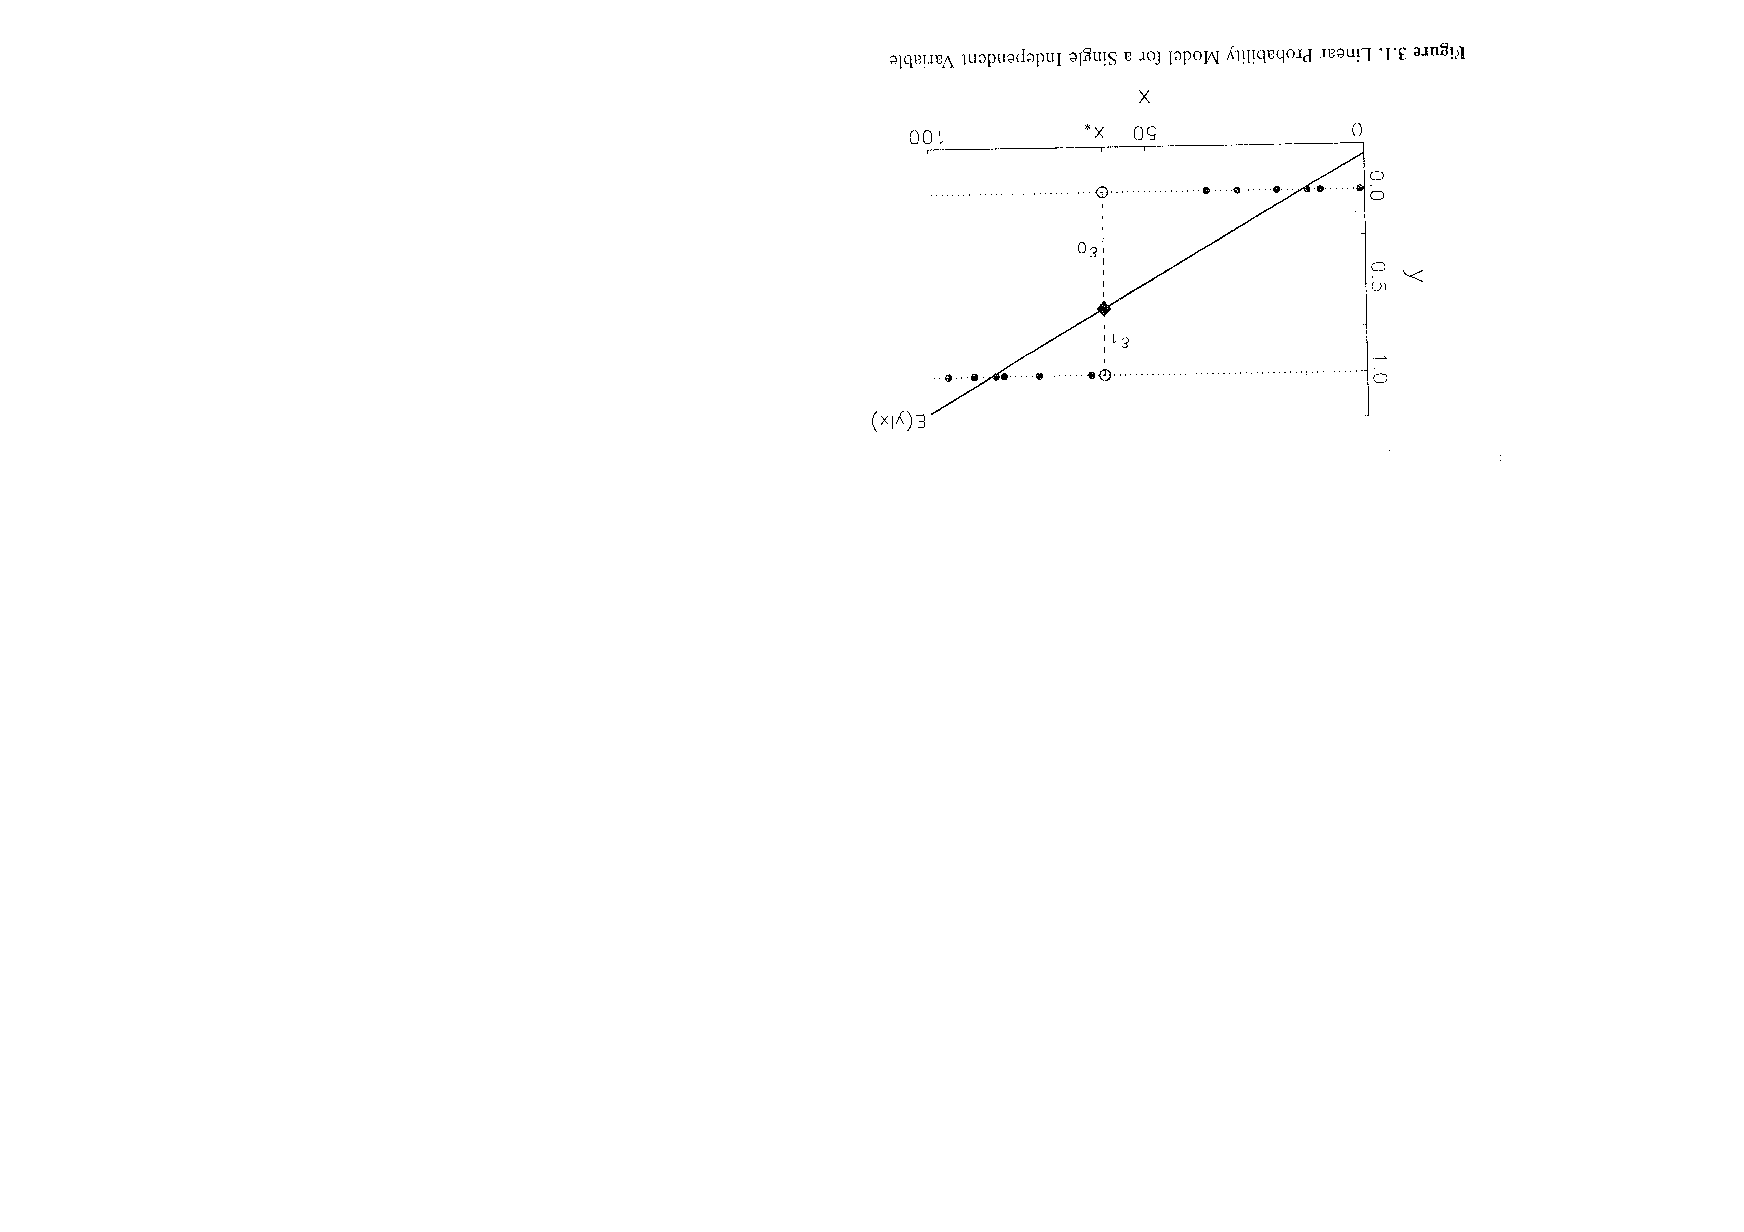
\includegraphics[angle=180,scale=.85]{graphs/sl_fig31.pdf}
\end{figure}
\end{center}
 }


\begin{frame}
\frametitle{Non-linear Probability Models}
LPM is easy to estimate and interpret. However, predicted probabilities may be non-sensical ($<0$ or $>1$).\medskip

Solution: approximate $P(Y_i=1|X_i)$ with some c.d.f.
\begin{eqnarray*}
  P(Y_i=1|X_i) = F(X_i \beta)
\end{eqnarray*}
$F()$ is a cumulative distribution function, $F\in[0,1]$ by definition.
\begin{itemize}
  \item $F=\Lambda$ logistic distribution c.d.f \emph{logit model}
  \item $F=\Phi$ normal distribution c.d.f \emph{probit model}
\end{itemize}
\end{frame}

 \frame{ 
\begin{center}
\begin{figure}[t]
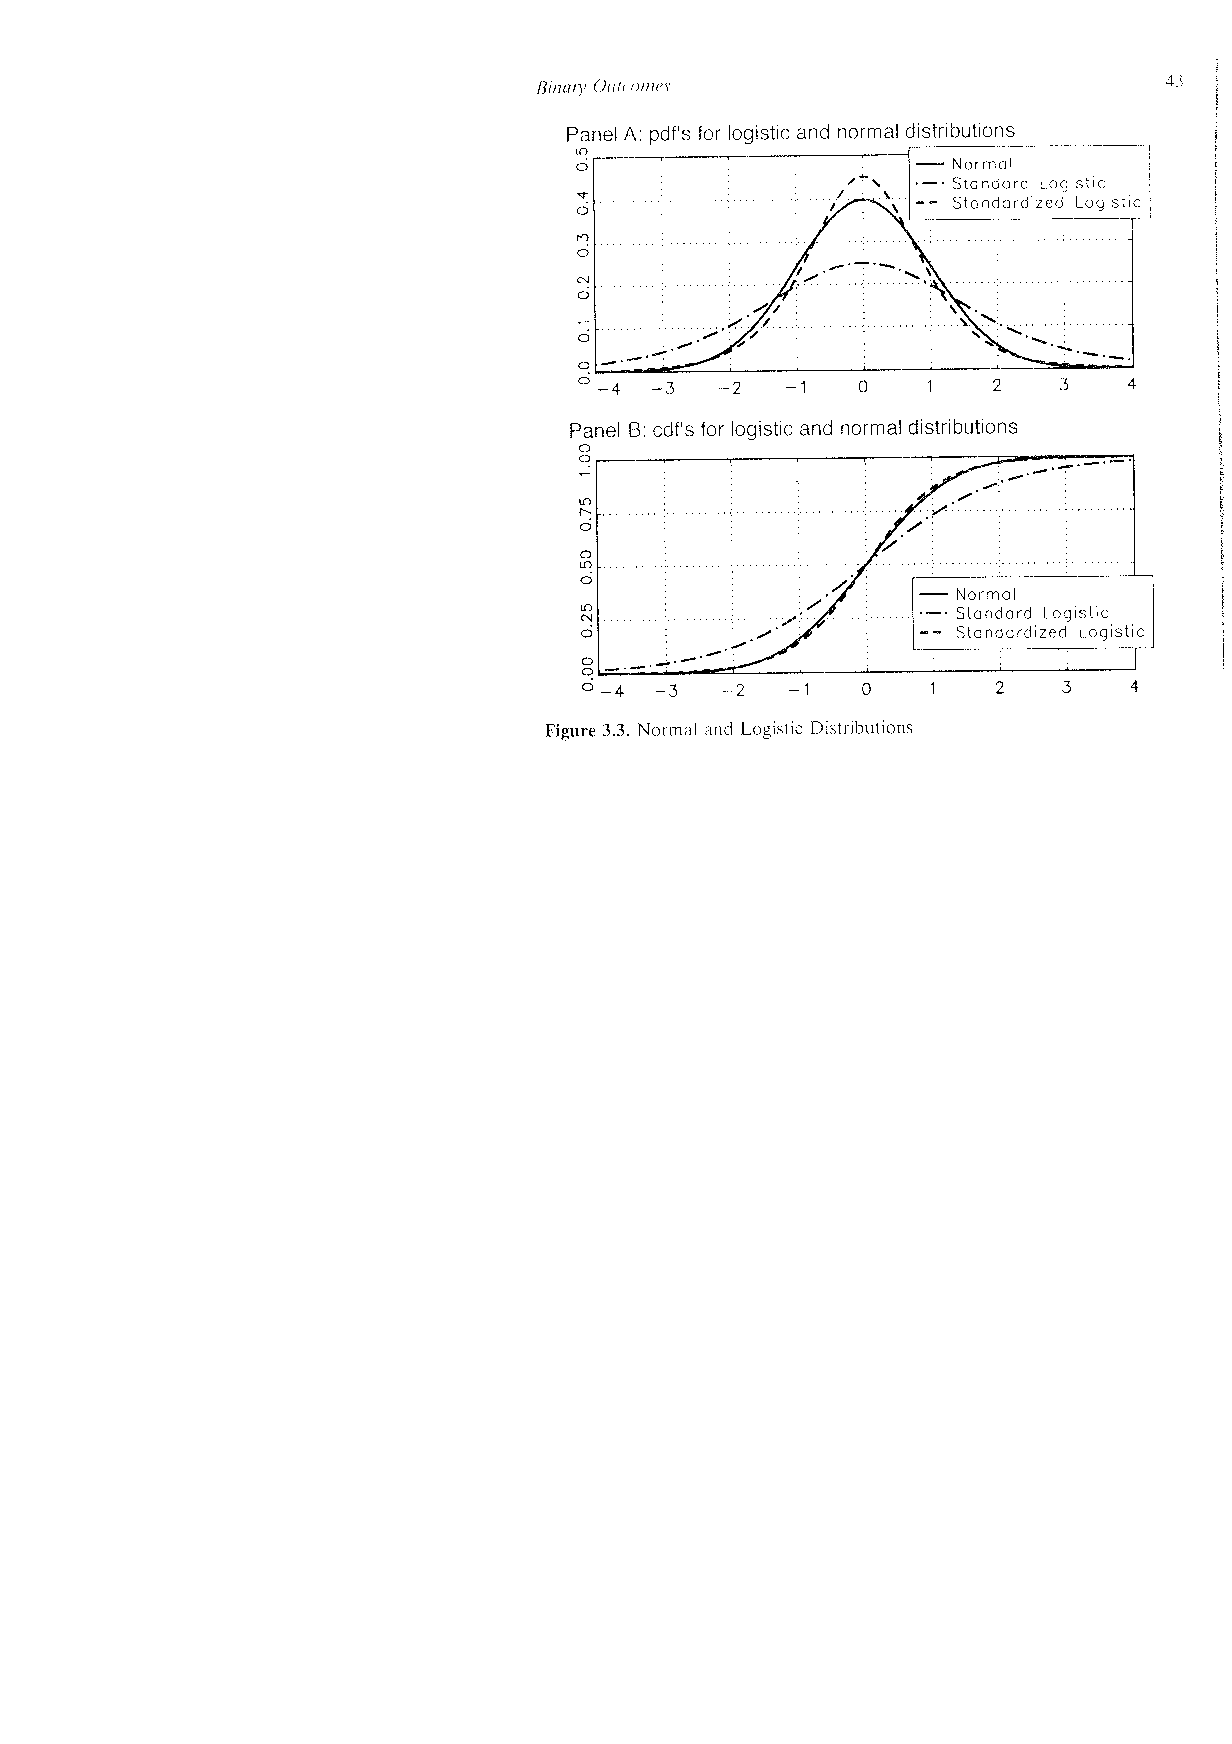
\includegraphics[angle=0,scale=.55]{graphs/sl_fig33.pdf}
\end{figure}
\end{center}
 }
 
% \begin{frame}
%\frametitle{Logit Model}
%
%\begin{eqnarray*}
%0 \leq  P(Y_i=1|X_i)\leq 1
%\end{eqnarray*}
%Transform the probability into a function that ranges between $-\infty$ and $\infty$.
%\begin{eqnarray*}
%% \nonumber to remove numbering (before each equation)
% 0 &\leq& \frac{ P(Y_i=1|X_i)}{P(Y_i=0|X_i)} = \frac{ P(Y_i=1|X_i)}{1-P(Y_i=1|X_i)}  \leq  \infty \\
% -\infty &\leq& log \left(\frac{ P(Y_i=1|X_i)}{1-P(Y_i=1|X_i)}\right) \leq  \infty \\
%\end{eqnarray*}
%\end{frame}
%
%
% \begin{frame}
%\frametitle{Logit Model}
%
%\begin{eqnarray*}
%log \left(\frac{ P(Y_i=1|X_i)}{1-P(Y_i=1|X_i)}\right) &=& E[Y_i|X_i] = X_i \beta \\
%\frac{ P(Y_i=1|X_i)}{1-P(Y_i=1|X_i)} &=&exp(X_i \beta) \\
%P(Y_i=1|X_i) &=&exp(X_i \beta) (1-P(Y_i=1|X_i))\\
%P(Y_i=1|X_i) &=&exp(X_i \beta) -exp(X_i \beta) P(Y_i=1|X_i)\\
%P(Y_i=1|X_i)&+&exp(X_i \beta) P(Y_i=1|X_i)=exp(X_i \beta) \\
%P(Y_i=1|X_i)(1&+&exp(X_i \beta))=exp(X_i \beta) \\
% P(Y_i=1|X_i)&=&  \frac{\exp(X_i \beta)}{1+\exp(X_i \beta)}=\Lambda(X_i \beta)
%\end{eqnarray*}
%\end{frame}




 \begin{frame}
\frametitle{Latent Variable Model}

\begin{eqnarray*}
  Y_i^* &=& X_i \beta + \varepsilon_i
\end{eqnarray*}
$ Y_i^*$ is continuous unobserved variable, "utility" from working.

We only observe the decision whether the individual is working
 \begin{eqnarray*}
 Y_i&=& \left\{ \begin{array}{cc}
                                               1 & \text{if}\;\; Y_i^* > 0 \\
                                                0 & \text{if}\;\; Y_i^* \leq 0
                                                 \end{array} \right.
\end{eqnarray*}
Model
\begin{eqnarray*}
  P(Y_i=1|X_i) = P(Y_i^* > 0 | X_i) &=& P(X_i \beta + \varepsilon_i > 0 | X_i) \\
  &=& P( \varepsilon_i > - X_i \beta  | X_i)
\end{eqnarray*}

\end{frame}


  \begin{frame}
\frametitle{Probit as Latent Variable Model}

Assumption about the distribution of $\varepsilon_i$:
\begin{eqnarray*}
  \varepsilon_i|X_i &\sim& N[0,1]\\
  P(Y_i=1|X_i) &=& P( \varepsilon_i > - X_i \beta  | X_i) = \\
  &=& 1- \Phi ( -X_i \beta ) =\Phi ( X_i \beta ) \;\;\ \text{Probit model}
\end{eqnarray*}

\begin{itemize}
  \item Estimated parameters in the Probit model $\beta$
  \item Fixed error variance $\sigma^2_{\varepsilon}=1$, less flexible than OLS.
\end{itemize}

\end{frame}

  \begin{frame}
\frametitle{Estimation of Binary Response Models}


\begin{description}
  \item[linear model] $\min S(\beta) = \sum (Y_i-X_i \beta)^2$

  We can solve the least squares problem analytically
  \item[non-linear model] $\min S(\beta) = \sum (Y_i-F(X_i \beta))^2$

  Non-linear least squares
    \item[Maximum likelihood] joint probability distribution of the data is treated as function of the unknown parameters
 \begin{eqnarray*}
  L(\beta) &=& P(\text{observe} (y_1,x_1)\text{and} (y_2,x_2) \text{and} ...(y_n,x_n)|\beta) \\
  \hat{\beta}_{ML} &=& \max_{\beta} L(\beta)
  \end{eqnarray*}   

  Chooses the most plausible parameter $\hat{\beta}_{ML}$ given the data
\end{description}
\end{frame}

  \begin{frame}
\frametitle{Parameter Interpretation}

Compare 2 models
\begin{description}
  \item[linear model]
  \[ Y_i = \alpha + X_i \beta + \delta D_i \]

  \item[non-linear model]
   \[ Y_i = F(\alpha + X_i \beta + \delta D_i) \]

\end{description}
\end{frame}

\frame{\frametitle{Linear Model}
\begin{center}
\begin{figure}[t]
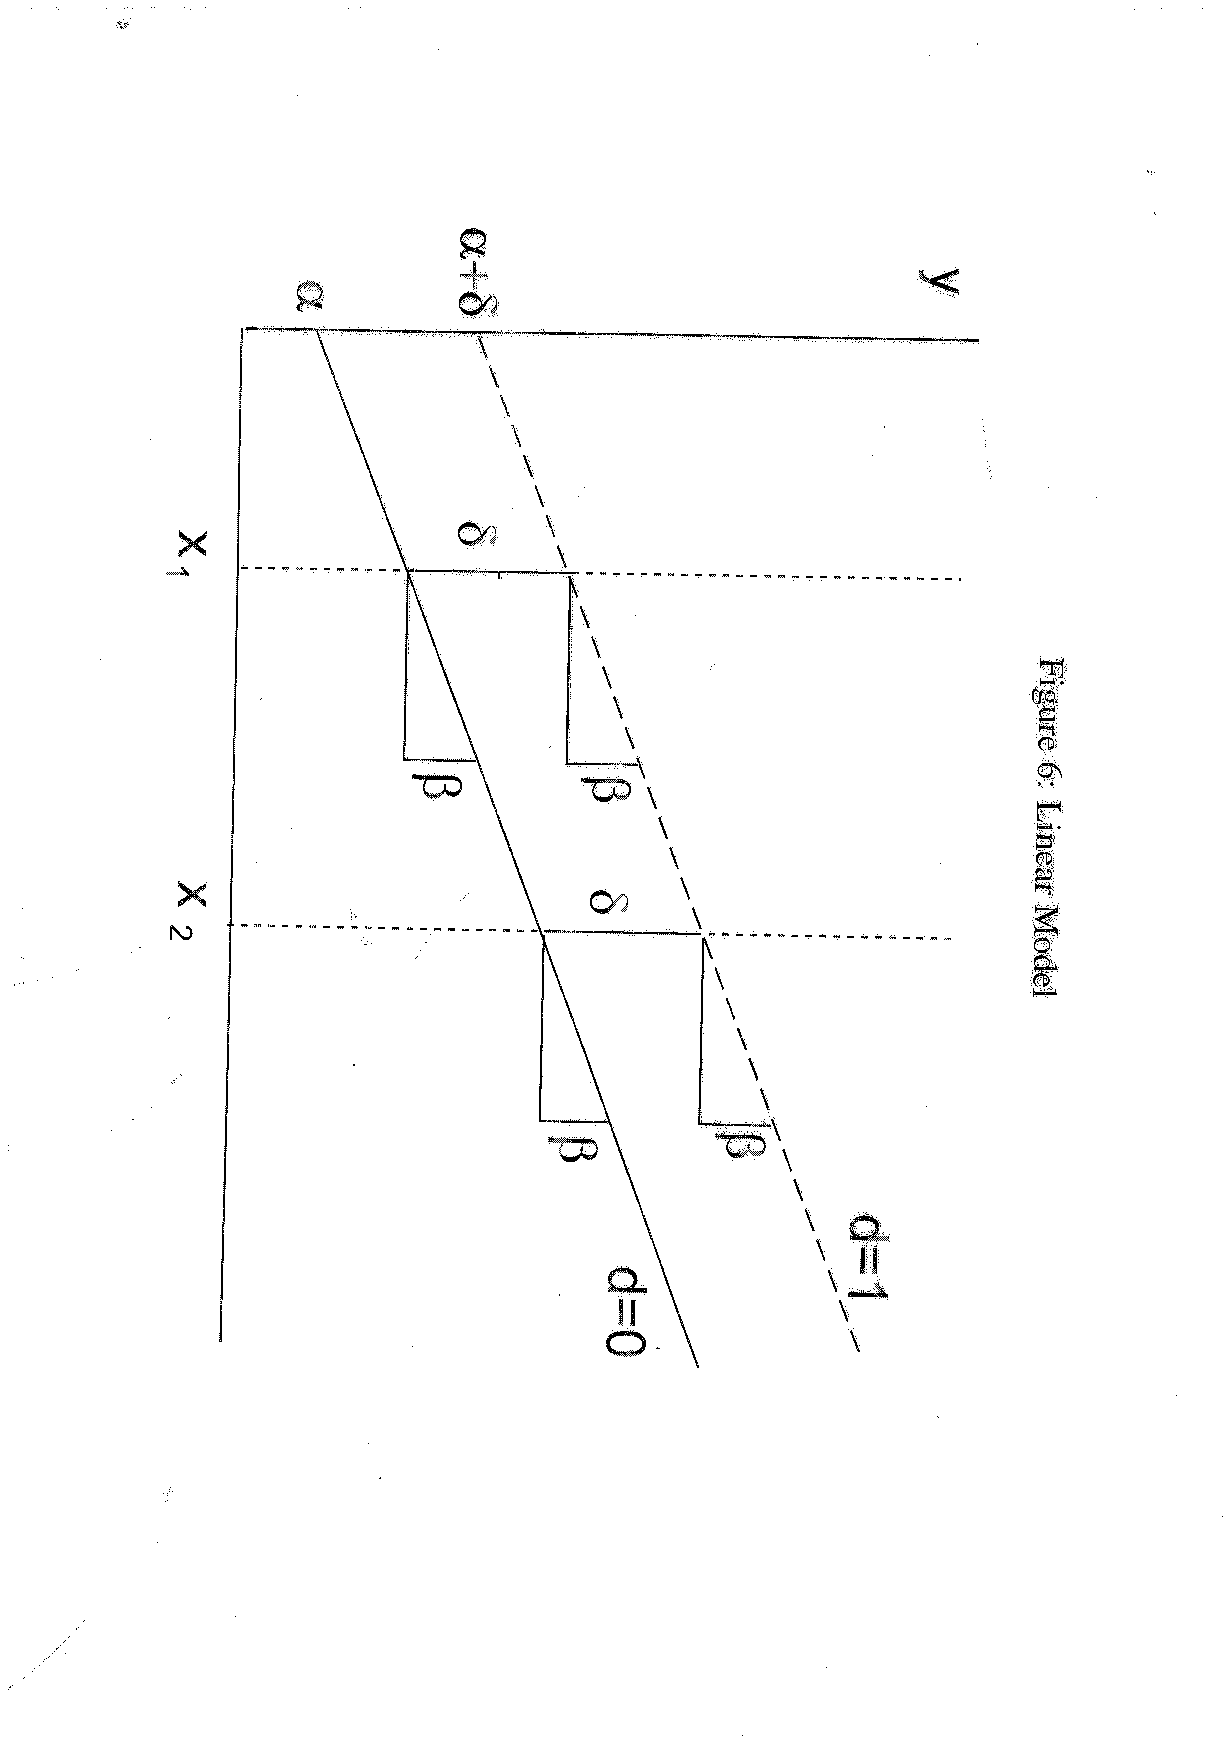
\includegraphics[angle=90,scale=.4]{graphs/sl_fig6.pdf}
\end{figure}
\end{center}
 }

  \frame{ \frametitle{Non-linear Model}
\begin{center}
\begin{figure}[t]
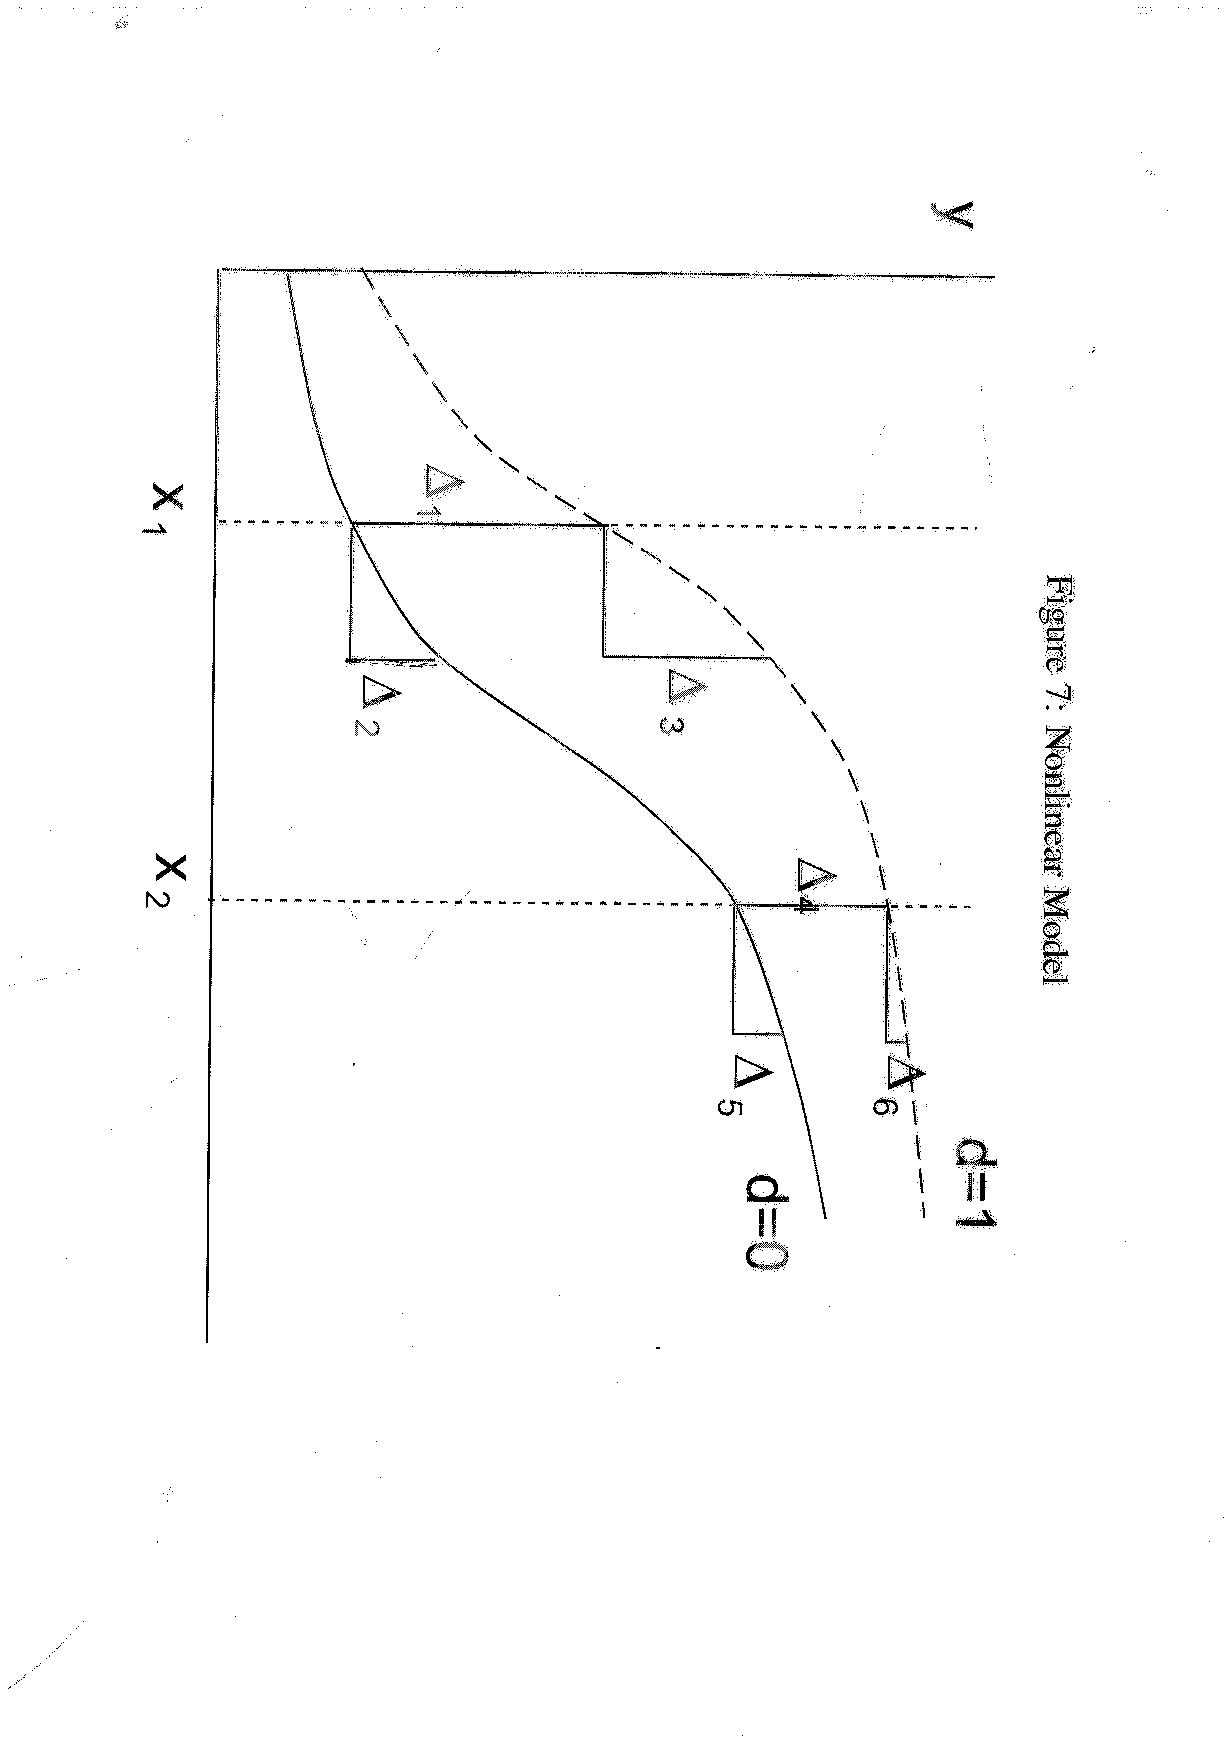
\includegraphics[angle=90,scale=.4]{graphs/sl_fig7.pdf}
\end{figure}
\end{center}
 }


\begin{frame}
\frametitle{Partial Change, Marginal Effect}

\begin{itemize}
  \item $Y = \alpha + X \beta + \delta D$, $\frac{\partial Y}{\partial X}=\beta$
  \item Partial effect in the non-linear model
  \begin{equation*}
    \frac{\partial P(Y_i=1|X )}{\partial X}= \frac{\partial F(X \beta)}{\partial X} \ast  \frac{\partial X \beta}{\partial X} = f(X \beta)\beta
  \end{equation*}
 \item  Marginal effect
 \begin{itemize}
   \item $\text{mean}\left(\frac{\partial P(Y=1|X_i)}{\partial X_i} \right)$
   \item $  \frac{\partial P(Y=1|X_i)}{\partial X_i}|_{X_i=\bar{X}}$
 \end{itemize}
\item  Discrete change (effect of dummy variable $D$)
\begin{itemize}
   \item $\frac{\Delta P(Y=1|D)}{X, \Delta D} = P(Y_i=1|X, D=1 ) - P(Y_i=1|X, D=0 )  $
 \end{itemize}
 
 \end{itemize}
\end{frame}


  \begin{frame}
\frametitle{Parameter Interpretation}

\begin{itemize}
  \item In the non-linear model the effect of $X_i$ or $D_i$ on $Y_i$ is not constant across different values of $X_i$ and $D_i$
  \item We can always interpret the sign and significance level of $\beta$ and $\delta$
  \item Scale of estimated parameters. Probability distributions are maximized at zero. 
  \begin{itemize}
    \item Logit: $f(0)=\frac{exp(0)}{[1+exp(0)]^2}=0.25$
    \item Probit: $f(0)=\frac{1}{\sqrt{2 \pi}} \approx 0.4$
    \item $\beta_l  \approx 1.6 \beta_p$
  \end{itemize}
  \item Investigate predicted probabilities: plots, $\min \hat{p}(Y_i=1|X_i)$,  $\max \hat{p}(Y_i=1|X_i)$
\end{itemize}
\end{frame}

\begin{frame}
\frametitle{Other questions to consider}
\begin{enumerate}
	\item{What if $\varepsilon_i$ in the latent utility is $N[0,\sigma]$, $\sigma\neq{1}$? Can we identify $\beta$ and $\sigma$?}
	\item{Heteroskedasticity: what if $\varepsilon_i$ in the latent utility is $N[0,\sigma(X)]$?}
\end{enumerate}

\end{frame}

\begin{frame}{Tobit}
Suppose the outcome of interest has a corner solution.\\\smallskip

Tipping cab drivers in NYC:
\begin{center}
	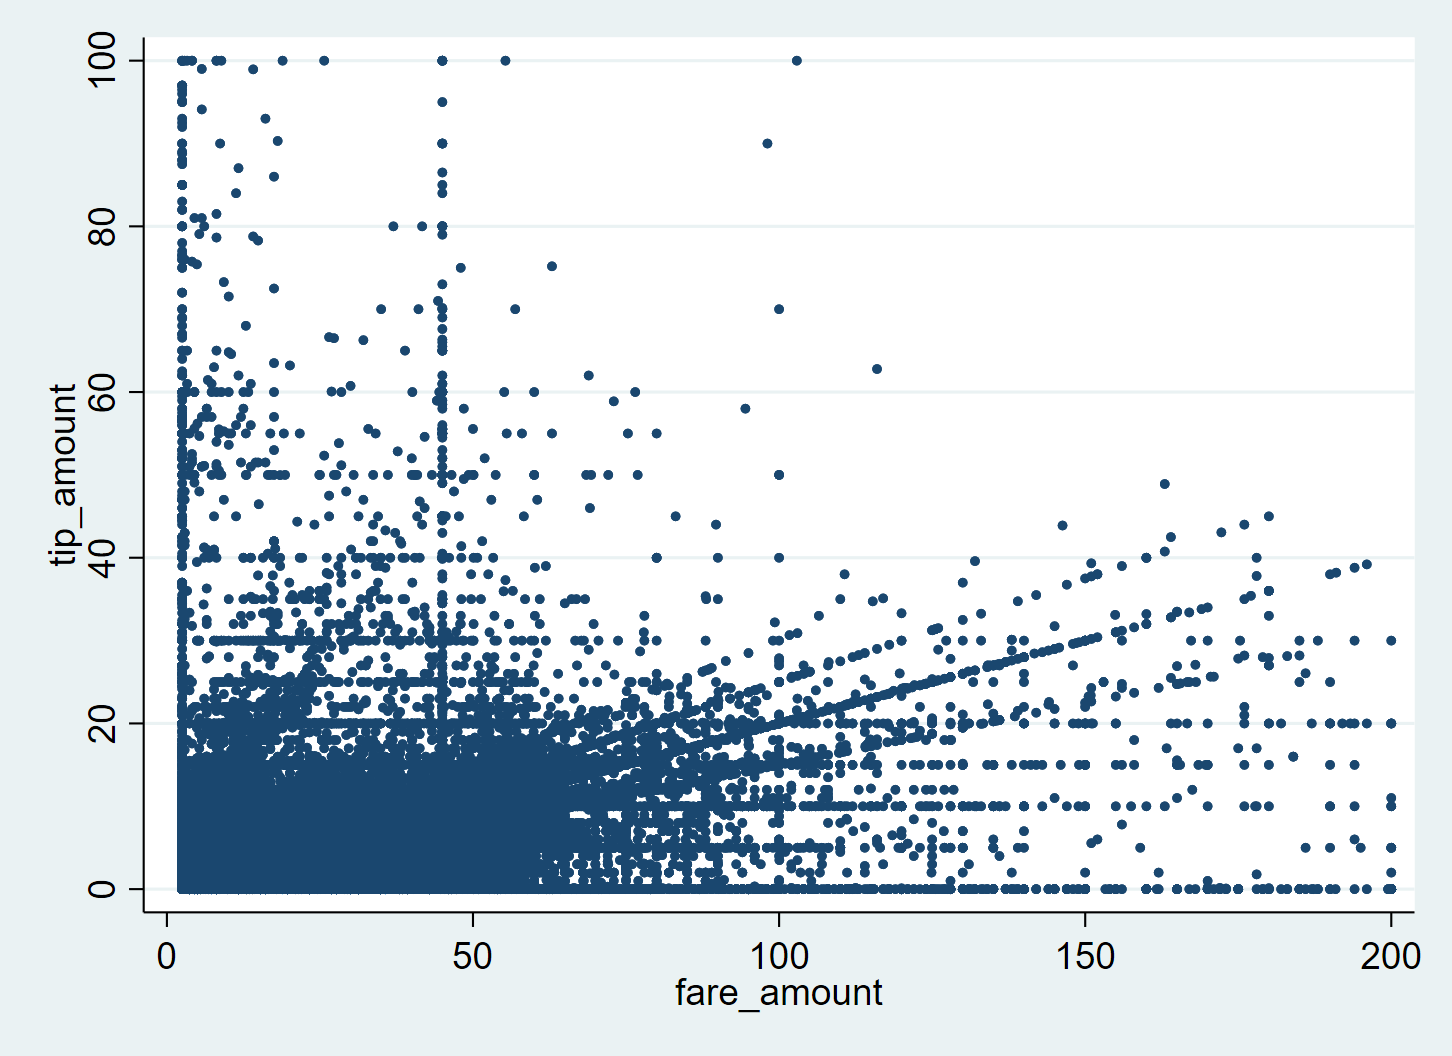
\includegraphics[width=0.7\textwidth]{graphs/cab_fares.png}
\end{center}
Many zeros; some passengers don't tip.
\end{frame}

\begin{frame}{True relationship vs what OLS estimates}
How does $X$ (total fare) affect expected tip, $E[Y|X]$?
\begin{center}
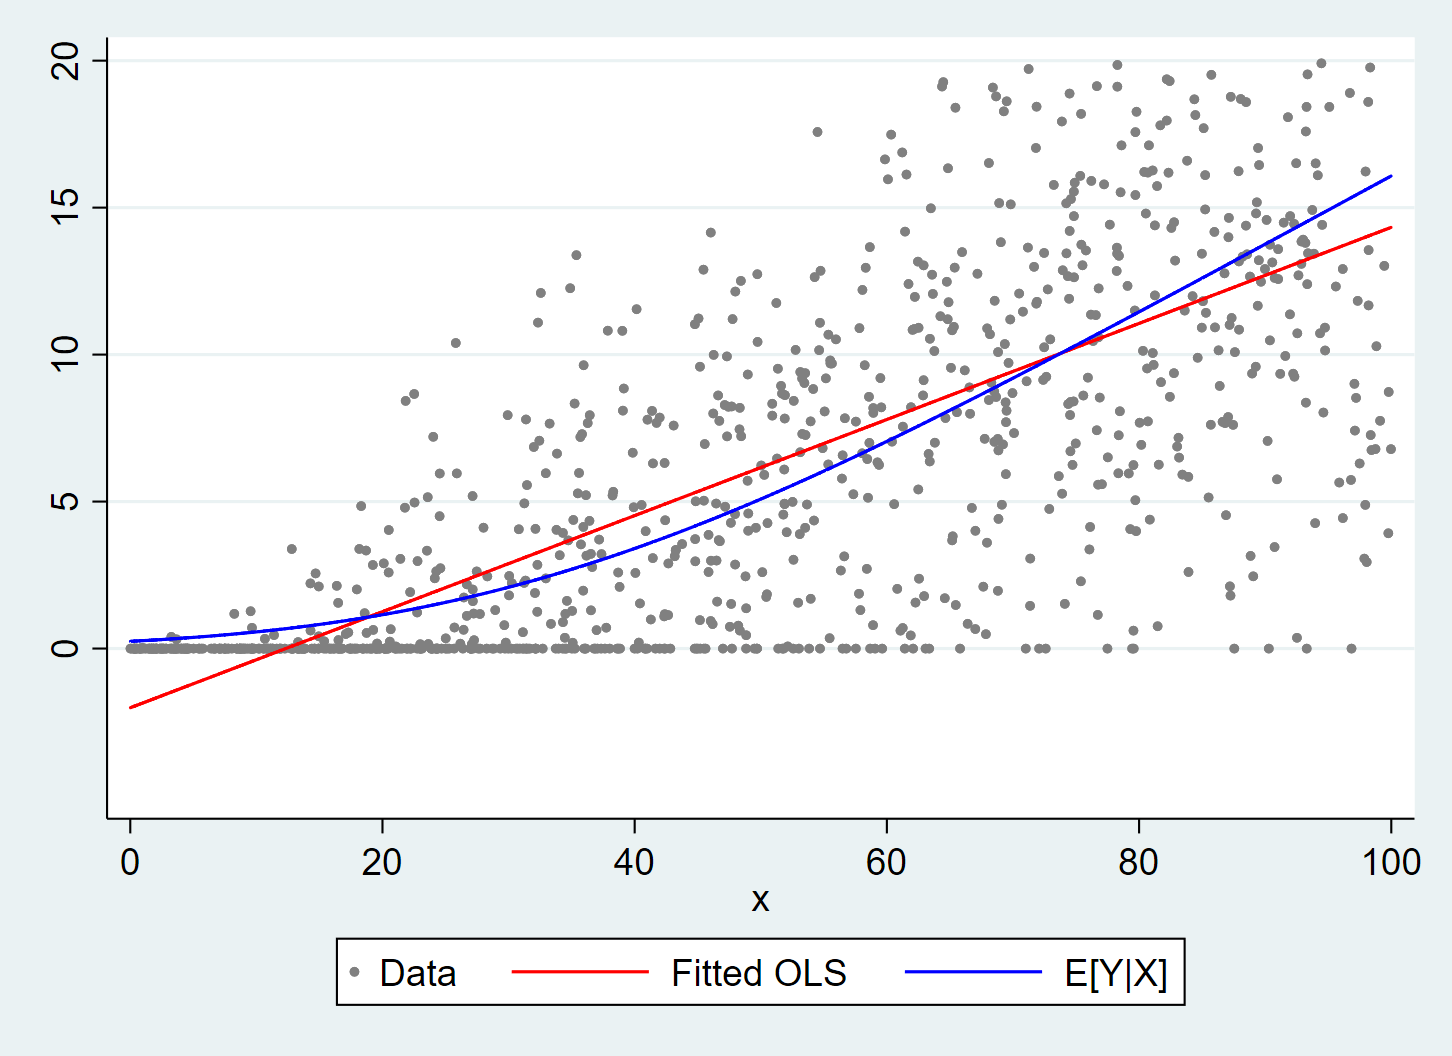
\includegraphics[width=0.8\textwidth]{graphs/ols_vs_tobit.png}
\end{center}

\end{frame}

\begin{frame}{True relationship vs what OLS estimates}
What's wrong with OLS here?
\begin{enumerate}
	\item OLS overestimates the effect for short trips.
	\item Vice versa for long trips.
	\item Issues with prediction (negative tips?).
\end{enumerate}
\end{frame}

\begin{frame}{Tobit}
Latent outcome --- tip one would like to pay
\begin{equation*}
	Y_i^* = X_i\beta + \varepsilon_i,\quad \varepsilon_i\sim{}N[0,\sigma]
\end{equation*}
Observed outcome --- actual tip: $Y_i = \max\{0, Y_i^*\}$. Parameters to estimate: $\beta$ and $\sigma$.
\begin{center}
	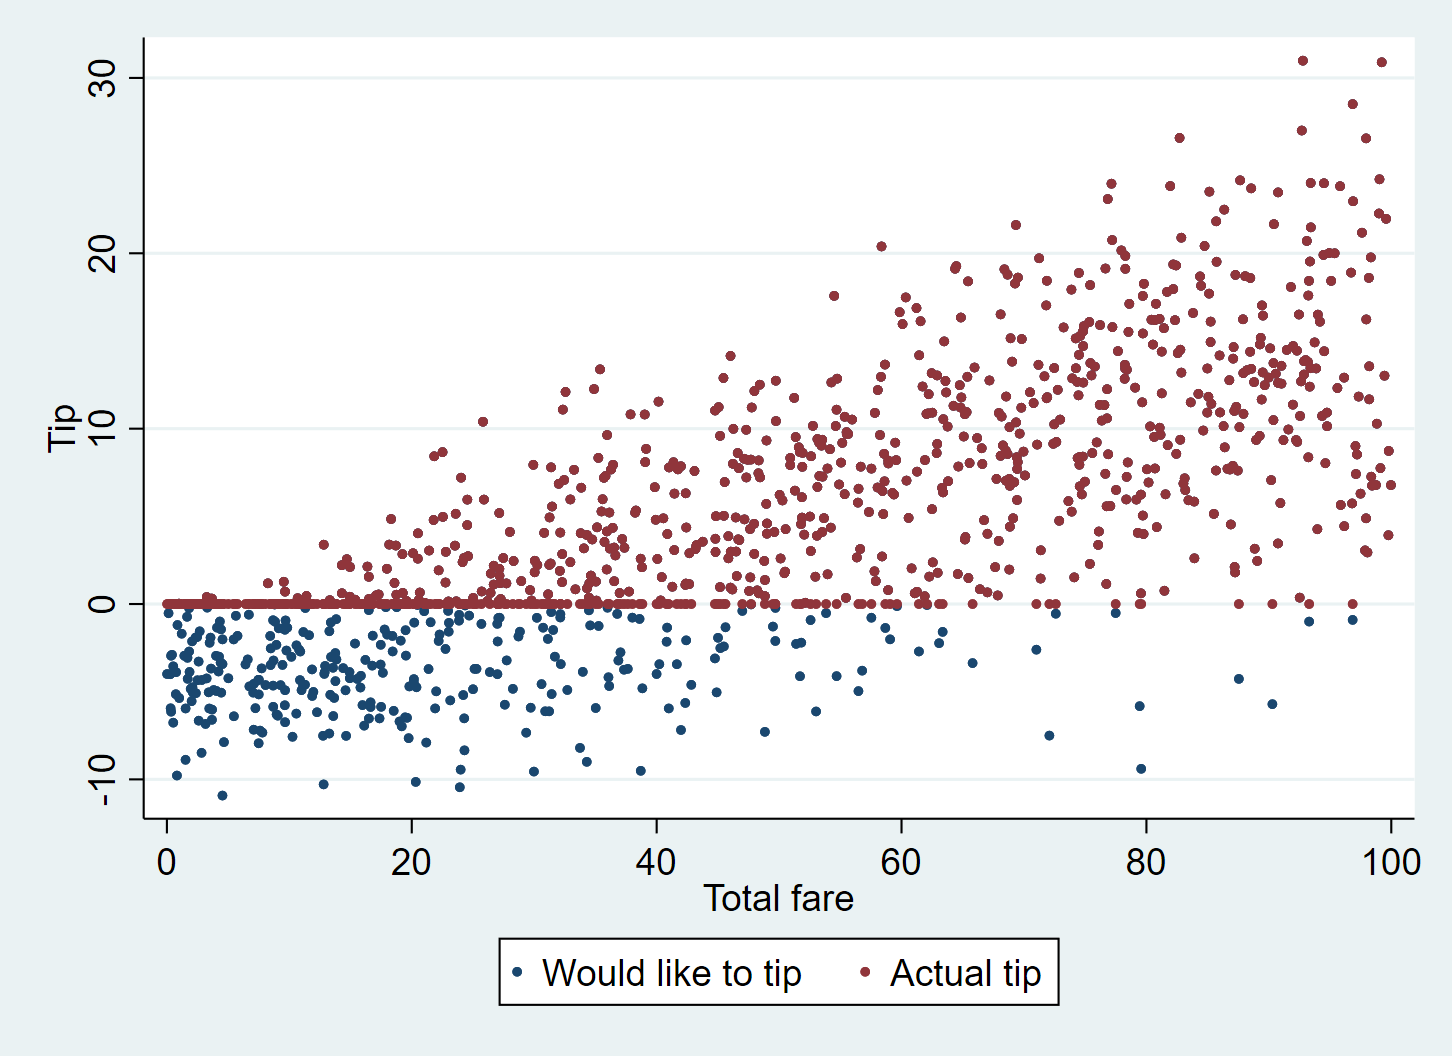
\includegraphics[width=0.75\textwidth]{graphs/tobit_latent_vs_actual.png}
\end{center}
\end{frame}

\begin{frame}{Estimating Tobit parameters}
Use ML; loglikelihood function:
\begin{align*}
	\ell&(\beta, \sigma; X, Y) = \sum_i\ell_i(\beta, \sigma; Y_i, X_i)\\
	&\text{where } \ell_i(\beta, \sigma; Y_i, X_i) = 
		\left\{
			\begin{array}{ll}
				\log{}P(Y_i=0|X_i), &\text{if $Y_i=0$,}\\
				\log{}f_\varepsilon(Y_i-X_i\beta), &\text{otherwise.}
			\end{array}
		\right.
\end{align*}
In Stata, run 
\begin{center}
	\texttt{tobit Y X, ll(0)}
\end{center}
\texttt{ll} stands for lower limit; can be different from zero.
\end{frame}

\begin{frame}{Interpreting the estimates}
We want to know $\dfrac{\partial{}E[Y|X]}{\partial{}X}$. But what is $E[Y|X]$?
\begin{align*}
E[Y|X] &= P(Y=0|X)\times{}0 + P(Y>0|X)E[Y|Y>0, X]\\
	&= \Phi\left(\frac{X\beta}{\sigma}\right)E[Y|Y>0, X]\\
	&= \Phi\left(\frac{X\beta}{\sigma}\right)\left\{X\beta + E[\varepsilon|\varepsilon>-X\beta]\right\}
\end{align*}
Since $\varepsilon$ is truncated normal, $E[\varepsilon|\varepsilon>-X\beta] = \sigma\phi\left(\frac{X\beta}{\sigma}\right)\left/\Phi\left(\frac{X\beta}{\sigma}\right)\right.$
\begin{equation*}
	E[Y|X] = \Phi\left(\frac{X\beta}{\sigma}\right)X\beta + \sigma\phi\left(\frac{X\beta}{\sigma}\right)
\end{equation*}
Marginal effects: $\dfrac{\partial{}E[Y|X]}{\partial{}X} = \Phi\left(\dfrac{X\beta}{\sigma}\right)\beta$
\end{frame}

\begin{frame}{Tobit. Concluding remarks}
\begin{itemize}
	\item Beware of rigid assumptions: error is normal r.v. with constant variance.
	\item Constant variance assumption can be relaxed
	\item Truncated and censored regression --- very similar concepts, slight differences in interpretation.
\end{itemize}
\end{frame}

\begin{frame}{Poisson regression}
	Two use cases:
	\begin{enumerate}
		\item Count outcomes: childbirths, arrests, number of cars in the family.
		\item \textbf{Continuous} non-negative dependent variable with skewed distribution and a mass point at zero.
	\end{enumerate}
\end{frame}

\begin{frame}{Poisson regression}
The outcome $Y_i$ counts events (e.g., number of times woman $i$ gave birth). Let $\theta_i = \exp(X_i\beta)$ approximate the ``rate of arrival''. Higher $\theta_i$ $\to$ high draws of $Y_i$ are more likely:
\begin{align*}
	P(Y_i=0|\theta_i) &= \exp(-\theta_i),\\
	P(Y_i=1|\theta_i) &= \theta_i\exp(-\theta_i),\\
	\dots\\
	P(Y_i=k|\theta_i) &= \frac{\theta_i^k}{k!}\exp(-\theta_i),\\
	\dots\\
	E[Y_i|\theta_i] &= \theta_i = \exp(X_i\beta)
\end{align*}
\end{frame}

\begin{frame}{Poisson regression -- How to Estimate and Interpret}
	\begin{itemize}
		\item\textbf{Estimation ---} ML: $\max_\beta\sum_i\left[Y_iX_i\beta - \exp(X_i\beta)\right]$.
		
		In Stata:
		\begin{center}
			\texttt{poisson Y X, vce(robust)}
		\end{center}
		Robust errors --- in case the model is slightly misspecified.
		\item\textbf{Interpretation:}
		\begin{equation*}
			\frac{\partial{}E[Y_i|X_i]}{\partial{}X_i} = \exp(X_i\beta)\beta
		\end{equation*}
		Marginal effects vary across $i$, but we know how to deal with this: use average marginal or evaluate the effect at $\bar{X}$.
	\end{itemize}
\end{frame}

\begin{frame}{Surprising application of Poisson regression}
	Gravity equation --- favorite tool of trade economists:
	\begin{align*}
		\log{EXPORTS_{od}} &= \alpha + \rho_1\log{GDP_o} + \rho_2\log{GDP_d}\\
			&-\beta{}TARIFF_{od} - \gamma\log{DIST_{od}} + \varepsilon_{od}
	\end{align*}
	Two issues:
	\begin{enumerate}
		\item $EXPORTS_{od} = 0$ for many country pairs. Typical shortcut: use a probit to model whether exports are non-zero.
		\item We are typically interested in the aggregate: $E[\sum_d{}EXPORTS_{od}]$.
	\end{enumerate}
	To find how tariffs affect exports: combine results from the export participation probit, the above gravity equation. Allow for the error in probit to correlate with the error in gravity, heteroskedasticity.\\\medskip
	
	Things get clunky very fast. Silva, Tenreyro (2006) --- use Poisson regression instead.
\end{frame}

\begin{frame}{Gravity and Poisson}
	Write gravity equation in levels rather than in logs:
	\begin{align*}
		E[EXPORTS_{od}] &= \exp\left(\alpha + \rho_1\log{GDP_o} + \rho_2\log{GDP_d}\right.\\
		 &- \left.\beta{}TARIFF_{od} - \gamma\log{DIST_{od}}\right)
	\end{align*}
	No logs --- no need to worry about zeros. 
	
	Use standard estimation routine; interpreting results is easy: effect of tariffs on total exports is 
	\begin{align*}
		\beta\sum_d\exp&\left(\alpha + \rho_1\log{GDP_o} + \rho_2\log{GDP_d}\right.\\
		 &- \left.\beta{}TARIFF_{od} - \gamma\log{DIST_{od}}\right)
	\end{align*}
	This works \textbf{even though exports are not discrete}. ML f.o.c. holds if $E[Y|X] = \exp(X\beta)$. $Y$ doesn't have to be Poisson r.v.!
\end{frame}

\begin{frame}{Sample Selection}
	Sample selection --- one of the major threats to identification. What types of selection cause trouble?
	\begin{enumerate}
		\item Random selection
		\item Selection on $X_i$
		\item Selection on $Y_i$ or $\varepsilon_i$
	\end{enumerate}
\end{frame}
\begin{frame}{Random selection}
	\begin{center}
		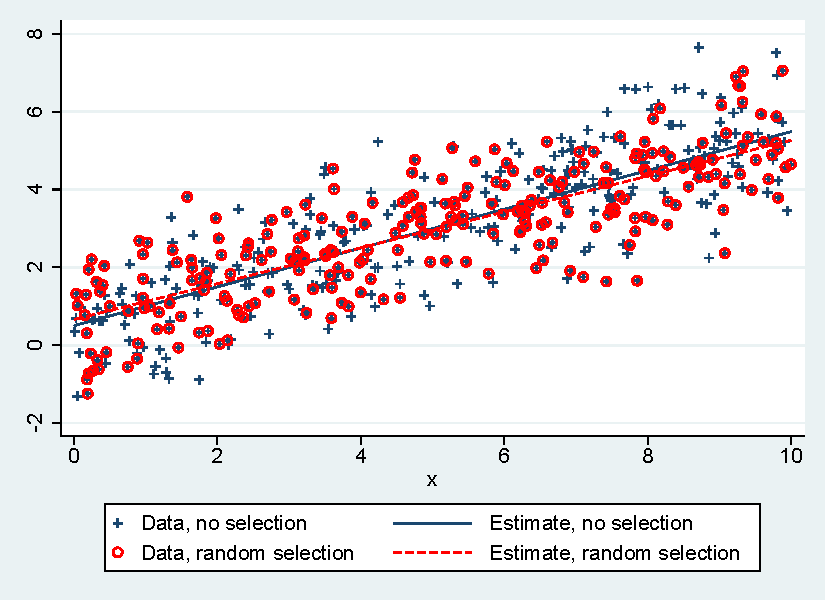
\includegraphics[width=0.9\textwidth]{graphs/selection_random.pdf}
	\end{center}
\end{frame}

\begin{frame}{Selection on controls}
\begin{center}
	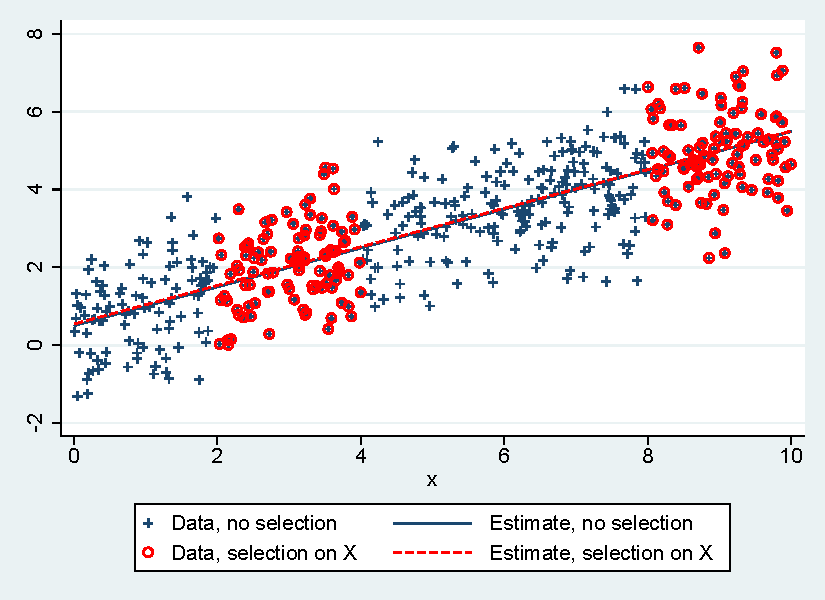
\includegraphics[width=0.9\textwidth]{graphs/selection_exog.pdf}
\end{center}
\end{frame}

\begin{frame}{Selection on unobservables/outcome}
\begin{center}
	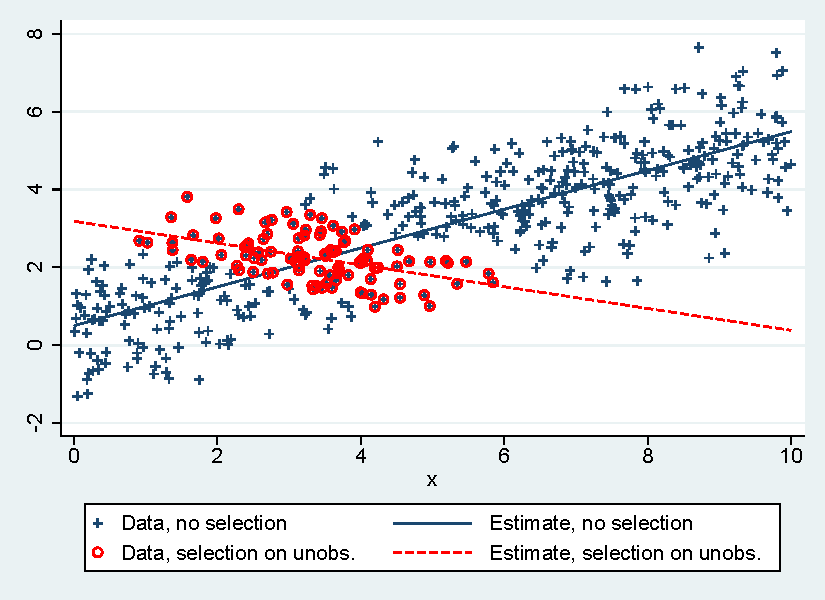
\includegraphics[width=0.9\textwidth]{graphs/selection_endog.pdf}
\end{center}
\end{frame}

\begin{frame}{More formal treatment}
	One way to think of selection:
	\begin{enumerate}
		\item{Draw random sample $i=1,..,N$.}
		\item{Apply random treatment $X_i$. Outcome $Y_i = X_i\beta + \varepsilon_i$}
		\item{Nature tosses a coin, $s_i\in\{0,1\}$. If $s_i = 1$, we observe $\{X_i, Y_i\}$. \textbf{Selected sample}: $\mathcal{S} = \{i : s_i=1, i=1,..,N\}$}
	\end{enumerate}
	Run OLS to estimate $\beta$ from
	\begin{equation*}
		Y_i = X_i\beta + \varepsilon_i, \quad i\in\mathcal{S}
	\end{equation*}
	or, use OLS for
	\begin{equation*}
		s_iY_i = s_iX_i\beta + s_i\varepsilon_i, \quad i=1,..,N
	\end{equation*}
	The results would be \textbf{identical}, but the latter is easier to study.
\end{frame}

\begin{frame}{Selection on controls}
OLS is a consistent estimator for $\beta$ in
\begin{equation*}
s_iY_i = s_iX_i\beta + s_i\varepsilon_i, \quad i=1,..,N
\end{equation*}
if $E[s_i\varepsilon_is_iX_i]=0$.\\\medskip
Is this the case under selection on controls?
\begin{align*}
	E[s_i\varepsilon_is_iX_i] &= E[s_iX_i\varepsilon_i]\\
	&= E\{E[E(s_iX_i\varepsilon_i|\varepsilon_i, X_i)|X_i]\}\\
	&= E\{X_iE[\varepsilon_iE(s_i|\varepsilon_i, X_i)]\}\\
	&= E\{X_iE[\varepsilon_ip(X_i)|X_i]\}\\
	&= E\{X_ip(X_i)E[\varepsilon_i|X_i]\}\\
	&= E\{X_ip(X_i)\cdot{0}\} = 0
\end{align*}
\end{frame}

\begin{frame}{Selection on unobservables. Heckman's method}
	What if selection is endogenous? Heckman's model:
	\begin{align*}
		Y_i &= X_i\beta + \varepsilon_i,\\
		s_i &\sim Probit: s_i = I[Z_i\gamma + \eta_i > 0]\\
		&(\varepsilon_i, \eta_i)|X_i,Z_i\sim{}N\left[0, \left[\begin{array}{cc}
			\sigma_\varepsilon^2, & \sigma_{\varepsilon\eta}\\
			\sigma_{\varepsilon\eta} & \sigma_{\eta}^2
		\end{array}\right]\right]
	\end{align*}
	\begin{itemize}
		\item{}In the canonical model, if $s_i=0$, we observe $(X_i, Z_i)$, but not $Y_i$.
		\item{}$s_i$ correlates with $\varepsilon_i$ via $\eta_i$. If $\sigma_{\varepsilon\eta} = 0$, selection is exogenous.
		\item{}Shocks are independent of $(X_i, Z_i)$ --- brave assumption!
	\end{itemize}
	
\end{frame}

\begin{frame}{Selection bias in Heckman's model}
	If you run $Y_i$ on $X_i$ for $i\in\mathcal{S}$, you are estimating
	\begin{align*}
		E[Y_i|X_i,Z_i, s_i=1] &= X_i\beta + \underbrace{E[\varepsilon_i| s_i=1, X_i,Z_i]}_{\text{selection bias}}\\
		&= X_i\beta + E[\varepsilon_i| \eta_i > -Z_i\gamma, X_i,Z_i]\\
		&\text{...tedious algebra...}\\
		&= X_i\beta + \frac{\sigma_{\varepsilon\eta}}{\sigma_\eta^2}E[\eta_i| \eta_i > -Z_i\gamma, X_i,Z_i]\\
		&\text{...more tedious algebra...}\\
		&= X_i\beta + \frac{\sigma_{\varepsilon\eta}}{\sigma_\eta}\frac{\phi\left(\frac{Z_i\gamma}{\sigma_\eta}\right)}{\Phi\left(\frac{Z_i\gamma}{\sigma_\eta}\right)}\\
		&= X_i\beta + \rho\lambda\left(\frac{Z_i\gamma}{\sigma_\eta}\right)
	\end{align*}
	where $\lambda(t) = \phi(t)/\Phi(t)$ --- inverse Mills ratio, $\rho$ --- constant.
\end{frame}

\begin{frame}{Heckman's two-step method}
\begin{enumerate}
	\item{Run probit, $s_i$ on $Z_i$, get $\widehat\gamma$. Find predicted $\widehat\lambda_i = \lambda(Z_i\widehat{\gamma})$.}
	\item{Run OLS, $Y_i$ on $X_i$ and $\widehat\lambda_i$; $\widehat\lambda_i$ absorbs selection bias.}
\end{enumerate}
Notes:
\begin{itemize}
	\item{Std. errors in the second step have to be corrected in a special way (since $\widehat\lambda\neq\lambda$). Use built-in commands, they do necessary corrections.}
	\item{Although $X_i = Z_i$ is allowed, find a control affecting $s_i$, but not $Y_i$. Otherwise $\lambda_i$ and $X_i$ may be highly collinear.}
	\item{But do not exclude controls from $X_i$ just because you want $Z_i$ to have more variables than $X_i$! You risk violating $\varepsilon_i\perp{Z_i}$}
\end{itemize}
\end{frame}

% \begin{frame}
%\frametitle{Probability of Marginal Employment}
%
%\renewcommand{\arraystretch}{1.0}
%\begin{tiny}
%
%\begin{table}[!htb]
%\begin{tabular}{llll}
%\hline\hline \\
%	 & 	        OLS	 & 	Logit & Probit	\\
%\hline		\\
%female	&	0.049	&	0.381	&	0.210	\\
%	&	(0.004)	&	(0.027)	&	(0.015)	\\
%age	&	0.001	&	0.009	&	0.005	\\
%	&	(0.000)	&	(0.002)	&	(0.001)	\\
%edu1	&	-0.083	&	-0.547	&	-0.310	\\
%	&	(0.010)	&	(0.069)	&	(0.039)	\\
%edu2	&	-0.087	&	-0.592	&	-0.335	\\
%	&	(0.010)	&	(0.068)	&	(0.039)	\\
%edu3	&	-0.066	&	-0.431	&	-0.243	\\
%	&	(0.011)	&	(0.078)	&	(0.045)	\\
%edu4	&	-0.020	&	-0.140	&	-0.075	\\
%	&	(0.012)	&	(0.081)	&	(0.047)	\\
%foreign	&	-0.042	&	-0.325	&	-0.183	\\
%	&	(0.005)	&	(0.038)	&	(0.021)	\\
%married	&	-0.010	&	-0.102	&	-0.053	\\
%	&	(0.003)	&	(0.026)	&	(0.015)	\\
%pdempl1	&	0.035	&	0.243	&	0.140	\\
%	&	(0.006)	&	(0.048)	&	(0.026)	\\
%mwage1	&	0.000	&	-0.001	&	0.000	\\
%	&	(0.000)	&	(0.000)	&	(0.000)	\\
%cons	&	0.276	&	-0.833	&	-0.546	\\
%	&	(0.013)	&	(0.097)	&	(0.054)	\\
%	&		&		&		\\
%N	&	51619	&	51619	&	51619	\\
%log-Likelihood	&		&	-21917	&	-21923	\\
%R-squared	&	0.033	&	0.038	&	0.038	\\
%correctly predicted	&		&	83.88\%	&	83.89\%	\\
%	&	56\%	&	60\%	&	59\% 	\\ \hline		\\
%\end{tabular}
%\end{table}
%\end{tiny}
%\end{frame}
%
%
%
%\begin{frame}
%\frametitle{Duration Models}
%
%Survival-time data or time-to-event data measures transitions between different states over time
%
%Examples: married, non-married
%
%\hspace{1.5 cm} employed, unemployed, inactive
%
%\bigskip
%Here: single spell, single state data
%\end{frame}
%
%
%\begin{frame}
%\frametitle{Censoring}
%
%Total spell-length or exact start and end dates are known exactly, we only that the spell began or ended within some time interval
%\begin{itemize}
%  \item Right-censoring: start date is known, but the relevant event has not yet occurred
%  \item Left-censoring: start date of the spell is not observed
%\end{itemize}
%
%\bigskip
%Here: completed spells or incomplete spells (right-censoring)
%\end{frame}
%
%\begin{frame}
%\frametitle{Data issues}
%
%Measures of survival-time
%\begin{itemize}
%  \item Discrete time: survival time measured in years, months, weeks, ...
%  \item Continuous time
%\end{itemize}
%
%Two types of regressors
%\begin{itemize}
%  \item Fixed over time: e.g. gender, age at entry, ...
%  \item Time varying: e.g. number of kids, unemployment rate,...
%\end{itemize}
%
%\end{frame}
%
%\begin{frame}
%\frametitle{Models of Survival-Time}
%
%Problems with OLS
%\begin{itemize}
%  \item Censoring
%  \item Time-varying covariates
%\end{itemize}
%
%\bigskip
%Problems with Logit
%\begin{itemize}
%  \item model $P(Y_i < t_0 |X_i)$ for fixed $t_0$: loss of information
%\end{itemize}
%
%\end{frame}
%
%
%\begin{frame}
%\frametitle{Survival, Hazard, and Cumulative Hazards}
%\begin{itemize}
%\item The dependent T variable is assumed to have a probability distribution  $f(t)$
%
%\item Probability that duration time is less than $t$
%\[ F(t) = P(T \leq t) \]
% \item \textit{Survival function} is the probability surviving past $t$
%  \[ S(t)=1-F(t) = P(T>t) \]
% \item \textit{Hazard Rate} is the instantaneous rate of leaving the initial state per unit of time. Given that the event has not occurred yet what are the chances that it will occur? \[ \lambda(t)= \frac{f(t)}{1-F(t)}=\frac{f(t)}{S(t)} \]
%  %The Hazard Rate is the probability that the individual will experience the event at time $t$ while the individual is at risk for experiencing the event
%\end{itemize}
%\end{frame}
%
%
%
%\begin{frame}
%\frametitle{Estimators of Survivor and Hazard Functions}
%
%Non-parametric estimators: no functional form assumptions 
%
%\bigskip
%$t_1< t_2 < ... < t_k$ observed survival times in the data
%
%Define as:
%\begin{description}
%  \item[$d_j$] number of individuals who make a transition out of the state at $t_j$
%  \item[$m_j$] number of individuals whose observed duration is censored at $t_j$
%  \item[$n_j$] number of individuals at risk of making a transition at $t_j$
%  %censored or completed spells of duration $t_j$ or longer;  $ n_j= (m_j + d_j) + (m_{j+1}  + d_{j+1}) + ...  $
% \end{description}
% 
%\end{frame}
%
%
%\begin{frame}
%\frametitle{Example}
%
%\begin{center}\scriptsize
%  \begin{tabular}{  | c | c | c | c | c | c | c |}
%    \hline
%    time & At risk         & Events           & Censored               & Hazard                 & Cumulative   & Survival  \\  
% ($t_j$) &  ($n_j$) & ($d_j$)  &($m_j$)& $\lambda(t_j)=\frac{d_j}{n_j}$ & $\Lambda(t_j)$ & $S(t_j)$ \\ \hline
% 3 &  100                 & 10 & 3  & 10/100=0.1 & 0.1 & 1-0.1=0.9 \\ \hline
% 4 &  100-10-3  & 3   & 2  &  3/87    & 0.1+ 0.034 & 0.9*(1-0.134)\\ 
%    &  =87          &      &     &  =0.034 & =0.134      &  =0.87\\ \hline
% 5 &  87-3-2  & 6   & 1  &  6/82    & 0.134+0.073 & 0.87*(1-0.073)\\ 
%    &  =82      &      &     &  =0.073 & =.207     &  =.806\\ \hline
%
%    \hline
%  \end{tabular}
%\end{center}
% 
%\end{frame}
%
%
%\begin{frame}
%\frametitle{Kaplan Meyer Survival Curve}
%
%Model the survival function by the following step-function
%  \begin{eqnarray*}
%  \hat{S}(t_1) &=& 1-P(t \leq t_1) = 1 - \frac{d_1}{n_1} \\
%  \hat{S}(t_2) &=& (1-P(t \leq t_1))(1-P(t_1 < t \leq t_2)) = (1 - \frac{d_1}{n_1}) (1 - \frac{d_2}{n_2}) \\
%  \vdots \\
%   \hat{S}(t_j) &=& \prod_{k=1}^{j} (1 - \frac{d_k}{n_k})
%  \end{eqnarray*}
%
%\begin{itemize}
%  \item Note: this method takes censored observations into account
%  \item Graphical method: plot $ \hat{S}(t_j)$ against time.
%\end{itemize}
% 
%\end{frame}
%
%
%
%
% \frame{ \frametitle{ }
%\begin{center}
%\begin{figure}[t]
%\includegraphics[angle=0,scale=.75]{graphs/LDV_fig1.pdf}
%\end{figure}
%\end{center}
% }
%
%
% \frame{ \frametitle{ }
%\begin{center}
%\begin{figure}[t]
%\includegraphics[angle=0,scale=.75]{graphs/LDV_fig2.pdf}
%\end{figure}
%\end{center}
% }
%
%
%\begin{frame}
%\frametitle{Regression Models}
%
%Regression analysis typically models hazard rates.
%
%Proportional hazard model, e.g. Cox-regression
%  \begin{eqnarray*}
%  \lambda(t_i,X_i) &=&  \lambda_0(t) exp(X_i \beta) 
%  \end{eqnarray*}
%  
% 
%
%\begin{itemize}
%  \item $\lambda_0(t)$ baseline hazard, change in hazard rate over time
%  \item $X_i$ are time-constant regressors
%  \item Cox: method to estimate coefficients $\beta$ without having to specify the baseline-hazard; semi-parametric method
%  \item Link to logit-model
%\end{itemize}
% 
%\end{frame}
%
\end{document}
%
%
%\end{document}
%
%
%
%
%\setlength{\itemsep}{.5 cm}
%
%  \frame{ 
%\begin{center}
%\begin{figure}[t]
%\includegraphics[angle=180,scale=.55]{graphs/sl_fig36.pdf}
%\end{figure}
%\end{center}
% }
%
%
%\begin{frame}
%\frametitle{Censored dependent variables}
%
%
%\end{frame}
%
%
%\frame{ \frametitle{Literature}
%\begin{itemize}
%  \item Rosenbaum, Paul R. and Donald B. Rubin (1984) "Reducing Bias in Observational Studies Using Subclassification on the Propensity Score" Journal of the American Statistical Association, 79, 516-524.
%  \item LaLonde, Robert J. (1986), "Evaluating the Econometric Evaluations of Training Programs with Experimental Data", American Economic Review 76, 604-620.
%  \item Dehejia, Rajeev H. and Sadek Wahba (1999) "Causal Effects in Nonexperimental Studies: Reevaluating the Evaluation of Training Programs" Journal of the American Statistical Association, 94, 1053-1062.
%  \item Imbens, Guido W. (2004) "Nonparametric Estimation of Average Treatment Effects Under Exogeneity: A Review" Review of Economics and Statistics, 86, 4-29.
%  \item Caliendo, Marco and Sabine Kopeinig (2008), "Some Practical Guidance for the Implementation of Propensity Score Matching" Journal of Economic Surveys, 22(1), 31-72.
%\end{itemize}



